\section{Abstract}

Data sets of immense size are regularly generated on large scale
computing resources.  Even among more traditional methods for
acquisition of volume data, such as MRI and CT scanners, data that is
too large to be effectively visualized on standard workstations is now
commonplace.

One solution to this problem is to employ a `visualization cluster,' a
small- to medium- scale cluster dedicated to performing visualization
and analysis of massive data sets generated on larger scale
supercomputers. These clusters are designed to fit a different
need than traditional supercomputers, and therefore their design
mandates different hardware choices, such as increased memory, and
more recently, graphics processing units (GPUs).  While there has
been much previous work on distributed memory visualization as well
as GPU visualization, there is a relative dearth of algorithms
that effectively use GPUs at a large scale in a distributed memory
environment.  In this work, we study a common visualization technique
in a GPU-accelerated, distributed memory setting, and present
performance charactersitcs when scaling to extremely large data sets.

\section{Introduction}
\label{sec:introduction}

Visualization and analysis algorithms, volume rendering in particular,
require extensive compute power relative to data set size.  One
possible solution is to use the large scale supercomputer that
generated the data, which clearly has the requisite compute power.
However it can be difficuilt to reserve and obtain the compute
resources required for viewing large data sets.  An alternative
approach, one explored in this work, is to use a smaller scale
cluster equipped with GPUs.  Such a cluster can provide the needed
computational power at a fraction of the cost---provided the GPUs
can be effectively utilized.  As a result, a semi-recent trend has
emerged to procure GPU-accelerated visualization clusters dedicated
to postprocessing the data generated by high-end supercomputers;
examples include ORNL's Lens, Argonne's Eureka, TACC's Longhorn, SCI's
Tesla-based cluster, and LLNL's Gauss.

Despite this trend, there have been relatively few efforts studying distributed
memory, GPU-accelerated visualization algorithms that can effectively utiliaze
the resources available on these clusters.  In this work, we report parallel
volume rendering performance characteristics on large data sets for a typ[ical
machine of this type.

Our system is divided into three stages:

\begin{enumerate}

  \item \emph{An intelligent pre-partitioning} that is designed to make
  combining results from different nodes easy.

  \item \emph{A GPU volume renderer} to perform per-frame volume
  rendering at interactive rates.

  \item \emph{MPI-based compositing} using a sort-last compositing framework.

\end{enumerate}

M\"uller et al. presented a system similar to our own that was limited
to smaller data sets~\cite{Needed}.  We have extended the ideas in that
system to allow for larger data sets, by removing the restriction that
a data set must fit in the combined texture memory of the GPU cluster
and adding the ability to mix in CPU-based renderers, enabling us to
analyze the parallel performance on extremely large data sets.  The
primary contribution of this component of our work is an increased
understanding of the performance characteristics of a distributed
memory GPU-accelerated volume rendering algorithm at a scale (256 GPUs)
much larger than previously published.  Further, the results presented
here (data sets up to $8192^3$ voxels) represent some of the largest
parallel volume renderings attempted thus far.

Our system and benchmarks allow us to explore issues such as:

\begin{itemize}

  \item the balance between rendering and compositing: a well-studied
  issue with CPU-based rendering, but currently with unclear
  performance tradeoffs for rendering on GPU clusters;

  \item the overhead of transferring data to and from a GPU;

  \item the importance of process-level load balancing; and

  \item the viability of GPU clusters for rendering very large data.

\end{itemize}

This chapter is organized as follows.  In Section~\ref{sec:previous},
we overview previous work in parallel compositing and GPU volume
rendering.  In Section~\ref{sec:arch}, we outline our system in detail.
Section~\ref{sec:eval} discusses our benchmarks and presents their
results. Finally, in Section~\ref{sec:conclusions} we draw conclusions
based on our findings.

\begin{figure}
  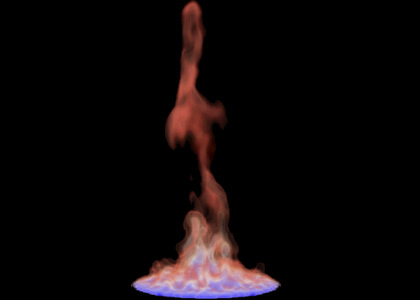
\includegraphics[width=\linewidth]{images/multiscale/teaser}
  \caption{Output of our volume rendering system with a data set
  representing a burning helium flame.}
  \label{fig:sample}
\end{figure}

\section{Previous work}
\label{sec:previous}

Volume rendering in a serial context has been studied for many years.
The
performance of the basic algorithm~\cite{Needed} was improved
significantly by incorporating empty space leaping and early ray
termination~\cite{Levoy:EarlyTermination}.  Max provided one of the
earliest formal presentations of the complete volume rendering equation
in~\cite{Needed}.  Despite significant algorithmic advances from
research such as~\cite{Levoy:EarlyTermination}, the largest increase in
performance for desktop volume renderers has come from taking advantage
of the 3D texture capabilities~\cite{Needed, Needed, Needed} and
programmable shaders~\cite{Krueger:2003:ATGV} available on modern
graphics hardware.

Extensive research has been done on parallel rendering and parallel
volume rendering.  Much of this work has focused on achieving
acceptable compositing times on large systems.  Molnar et al. conveyed
the theoretical underpinnings of rendering
performance~\cite{Molnar:199?:???}.  Earlier systems for parallel
volume rendering relied on direct send~\cite{Hsu:1993:???,
Ma:1993:???}, which divides the volume up into at least as many
chunks as there are processors, sending ray segments (fragments) to a
responsible tile node for compositing via the Porter and Duff
\emph{over} operator~\cite{PorterDuff:1984:Compositing}.  These
algorithms are simple to implement and integrate into existing systems,
but have sporadic compositing behavior and the potential to exchange a
large a number of fragments, straining the network layers when scaling
to large numbers of processors.  Tree-based compositing algorithms
feature more regular communication patterns, but impose an additional
latency that may not be required, depending on the particular frame
and data decomposition.  Binary swap and derivative algorithms are a
special case of tree-based algorithms that feature
equitable distribution of the compositing workload~\cite{Ma:1994:???}.
Despite advancements in compositing algorithms, network traffic remains
unevenly distributed in time, and thus high-performance networking
remains a necessity for subsecond rendering times on large numbers of
processors.

In the area of distributed memory parallel volume rendering of very
large data sets, the algorithm described by Ma et al
in~\cite{Ma:1993:???} has been taken to extreme scale in several
followuip publications.  In~\cite{Childs:2006:???}, data set sizes of
up to $3000^3$ are studied using hundreds of cores.  In this regime,
the time spent ray casting far exceeds the composite time.
In~\cite{PYRM:2008:???, PYR:2009:???}, the data set sizes range up to
$4480^3$, while core counts of tens of thousands are studied.
In~\cite{HBC:2010:???}, the benefits of hybrid parallelism are explored
at concurrency ranges going above two hundred thousand cores.  For both
of these studies, when going to extreme concurrency compositing time
becomes large and dominates ray-casting time.  This suggests that a
sweet spot may exist with GPU-accelerated distributed memory volume
rendering.  By using hardware acceleration, the long ray
casting times encountered in~\cite{Childs:2006:???} can be overcome.
Simultaneously, the emerging trend of composite-bound rendering
observed in~\cite{PYR:2009:???} and~\cite{HBC:2010:???} will be
mitigated by the ability to use many fewer nodes to command the same
compute power.

Numerous systems have been developed to enable parallel rendering in
existing software.  Among the most well-known is
Chromium~\cite{HHN:2002:???}, a rendering system that can transparently
parallelize OpenGL-based applications.  The Equalizer framework boasts
multiple compositing strategies, including an improved direct
send~\cite{EP:2007:???}.  The IceT library provides parallel rendering
with a variety of sort-last compositing strategies~\cite{MWP:2001:???}.

There has been less previous work studying volume rendering on
multiple GPUs.  Strengert et al. developed a system that used wavelet
compression and adaptively decompressed the data on small GPU
clusters~\cite{SMW:2004:???}.  Marchesin et al. compared a volume that
ran on two different two-GPU configurations: two GPUs on one system,
and one GPU on two networked systems~\cite{Marchesin:2008:MultiGPU}. The
use of just one or two systems, coupled with an in-core renderer,
artificially constrained the data set size.  M\"uller et al. developed
a distributed memory volume renderer that ran on
GPUs~\cite{Mueller:2006:???}; their system differs from ours in a few
key ways.  First, we use an out-of-core renderer and therefore can
exceed the available texture memory of the GPU by also utilizing CPU
memoryor disk.  To further reduce memory costs, we compute gradients
dynamically in the GLSL shader~\cite{KW:2003:???}, obviating the need
to upload a separate gradient texture.  This also has the benefit of
avoiding a pre-processing step, which is normally software-based in
existing general-purpose visualization applications (including the one
we chose to implement our system within) and can be time consuming for
large data sets.  Further differentiating our system and in line with
recent trends in visualization cluster architectures, we enable the use
of multiple GPUs per node.  M\"uller et al. used a direct send
compositing strategy~\cite{Hsu:1993:???, MPHK:1993:???}, whereas we use
a tree-based compositing method~\cite{MWP:2001:???}.  Finally, and
most importantly, we report performance results for substantially more
GPUs and much larger data sets, detailing the scalability of GPU-based
visualization clusters.  We therefore believe our work is the first
to evaluate the usability of distributed memory GPU clusters for this
scale of data.

\section{Architecture}
\label{sec:arch}

We implemented our remote rendering system inside of
VisIt~\cite{Childs:???:???}, which is capable of rendering data in
parallel on remote machines.  The system is comprised of a lightweight
`viewer' client application, connected over TCP to a server that
employs GPU cluster nodes.  All rendering is performed on the cluster,
composited via MPI, and images (optionally compressed via zlib) are
sent back to the viewer for display.  Example output from our system is
in Figure~\ref{fig:sample}.

Although VisIt provided a good starting point for our work, we needed
to make significant changes in order to implement our system.  In this
section, we highlight the main features of our system, taking special
care to note where we have deviated from existing VisIt functionality.

\subsection{Additions to VisIt}

\subsubsection{Multi-GPU access}

At the outset, VisIt's parallel server supported only a single GPU per
node.  We have revamped the manner in which VisIt accesses GPUs to
allow the system to take advantage of multi-GPU nodes.  When utilizing
GPU-based rendering, each GPU is matched to a CPU core that feeds
data to that GPU.  Additionally, when the number of CPU cores exceeds
the number of available GPUs, we allow for the use of software-based
renderers on the extra CPUs.  This code has been contributed to the
VisIt project.

\subsubsection{Partitioning}

VisIt contained a number of load decomposition stratgies prior to our
work.  However, we found these stratgies to be insufficient for a
variety of reasons:

\begin{enumerate}

  \item \textbf{Brick-based} Equalizing the distribution of work in
  VisIt was entirely based on \emph{bricks}, or pieces of the larger
  data set.  Our balancing algorithms use the time taken to render the
  previous frame to determine the weighted distribution of loads.

  \item \textbf{Master-slave} Dynamic balance algorithms in VisIt are
  based on a \emph{master} node that tells slaves to process a brick,
  waits for the slaves' completion, and then sends them a new brick to
  process.  We implemented a flat hierarchy, as seems to be more common
  in recent literature~\cite{Marchesin:2006:???, MSE06}.

  \item \textbf{Compositing} \emph{Most importantly}, for our
  object-based decomposition to work correctly, we needed a defined
  ordering to perform correct compositing.  The load balancing and
  compositing subsystems in VisIt were independent prior to our work.

\end{enumerate}

Our system relies on a \emph{k}d-tree for distributing and balancing
the data.  The spatial partitioning is done once initially and can
be adaptively refined by the rendering times from previous frames.
The initial tree only considers the number of bricks in the available
data set and attempts to distributed them evenly among processes, to
the extent that is possible.  When using static load balancing, this
decomposition is invariant for the life of the parallel job.
Figure~\ref{fig:decomposition} depicts a possible configuration
determined by the
partitioner, and shows the corresponding \emph{k}d-tree.

\begin{figure*}
  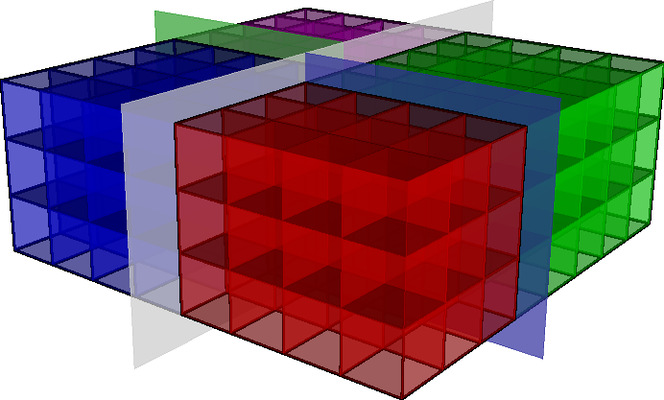
\includegraphics[width=0.49\linewidth]{images/multiscale/bricks.jpg}
  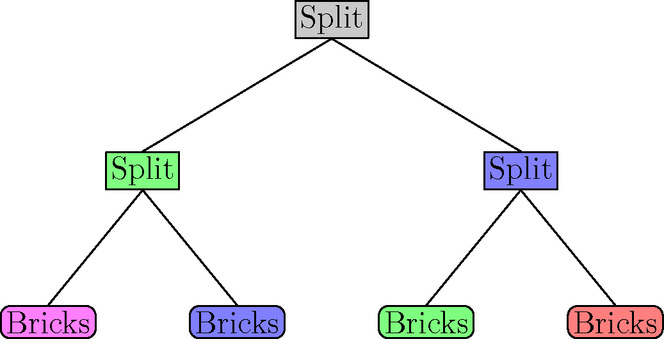
\includegraphics[width=0.49\linewidth]{images/multiscale/tree.jpg}
  \caption{Decomposition and corresponding kd-tree for an 8x8x3 grid
  of bricks divided among 4 processors.  Adjacent bricks are kept
  together for efficient rendering and compositing.  A composite order
  is derived dynamically from the camera location in relation to the
  splitting planes.  Note that the number of leaves in the tree is
  equal to the number of processes in the parallel rendering job.}
  \label{fig:decomposition}
\end{figure*}

When the dynamic load balancer is enabled, we use the last rendering
time on each process to determine the next configuration.  In our
initial implementation, the metric we utilized was the total pipeline
execution time to complete a frame.  This included the time to read
data from the disk, as well as the compositing time, among other
inputs.  However, we found that I/O would dwarf the actual rendering
time.  Further, compositing time is not dependent on the distribution
of bricks.  This therefore proved to be a poor metric.  Switching the
balancer to use the total render time for all bricks on that process
gave significantly better results.

In order to compare different implementations, we implemented multiple
load balancing algorithms, notably those described in Marchesin et al.
and M\"uller et al.'s work~\cite{Marchesin:2006:???, MSE06}.  In both cases, leaf
nodes represent processes, and each process has some number of bricks
assigned to it.  In the Marchesin-based approach, we start at the
parents of the leaf nodes and work our way up the tree, searching for
imbalance among siblings.  If two siblings are found to be imbalanced,
a single layer of bricks is moved along the splitting plane.  This
process continues up the root of the tree, at which time the virtual
results are committed and the new tree dictates the resulting data
distribution.  In the M\"uller-based approach, we begin with the root
node and use a pre-order traversal to find imbalance among siblings.
Once imbalance is found, the process stops for the current frame.
Instead of blindly shifting a layer of bricks between the siblings,
the method derives the average rendering cost associated with a layer
of bricks along the split plane, and shifts this layer if the new
configuration is projected to improve rendering time.

In addition to achieving a relatively even balance among the data, the
\emph{k}d-tree is used in the final stages to derive a valid sort-last
compositing order.

\section{Evaluation}
\label{sec:eval}

\todo{add / copy tbl:clusters from paper!!}

We implemented and tested our system on \textit{Lens}, a GPU-accelerated
visualization cluster housed at ORNL.  However, we were only able to access 16
GPUs on that machine.  In order to access a larger number of GPUs, we
transitioned to \textit{Longhorn}, a larger cluster housed at the Texas
Advanced Computing Cluster (TACC).  Specifications for each cluster are listed
in Table~\ref{tbl:clusters}.  Due to machine availability and configuration, we
were not able to fully utilize either machine.

\subsection{Rendering times}

The two dominant factors in distributed memory visualization
performance are the time taken to render the data and the time taken
to composite the resulting sub-images.  These have the largest impact
on usability because they comprise the majority of the latency a user
experiences: the time between when the user interacts with the data and
when the result of that interaction are displayed.

\begin{figure}
  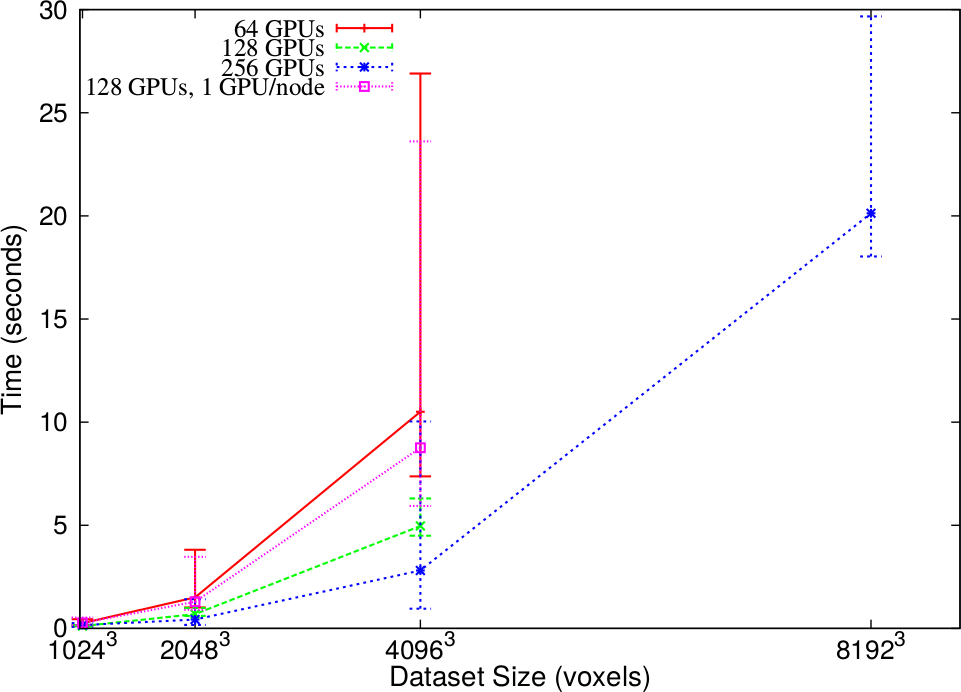
\includegraphics[width=\linewidth]{images/multiscale/rtime}

  \caption{Overal rendering time when rendering to a 1024x768 viewport
  on Longhorn.  This incorporates both rendering and compositing, and
  therefore shows the delay a user would experience if they used the
  system on a local network. Data points are the average across many
  frames, and error bars indicate the rendering timesor the slwoest and
  quickest frames, respectively.  For these results we used a domain
  consisteing of $13^3$ bricks (varying brick size) with the exceptions
  that all runs in the 128 GPU cases used $8^3$ bricks, and the run for
  the $8192^3$ data set was done using $32^3$ bricks.}
  \label{fig:rtime}
\end{figure}

Our data originated from a simulation performed by the Center for Simulation of
Accidental Fires and Exploisions (C-SAFE), desinged to study the instabilities
in a burning helum flame.  In order to study performance at varying
resolutions, we resampled this data to $1024^3$, $2048^3$, $4096^3$, and
$8192^3$, at a variety of bricks sizes.  We then performed tests, varying data
resolution, image resolution, choice of brick size, and number of GPUs, up to
256.  Unless noted otherwise, we divided the data into a grid of $8x8x8$ bricks
for parallel processing (larger data sets used larger bricks), and rendered
into a 1024x768 viewport.

Figure~\ref{fig:rtime} shows the scalability on the \textit{Longhorn}
cluster.  The principal input that affects rendering time is the data
set size, as one might expect.  These runs were all done using 2 GPUs
per node, except the ``128 GPUs, 1 GPU/node'' case, which was run on
128 nodes, each accessing a single GPU.  With very large data, there is
a modest increase in performance for this experimental setup.

\begin{figure}
  %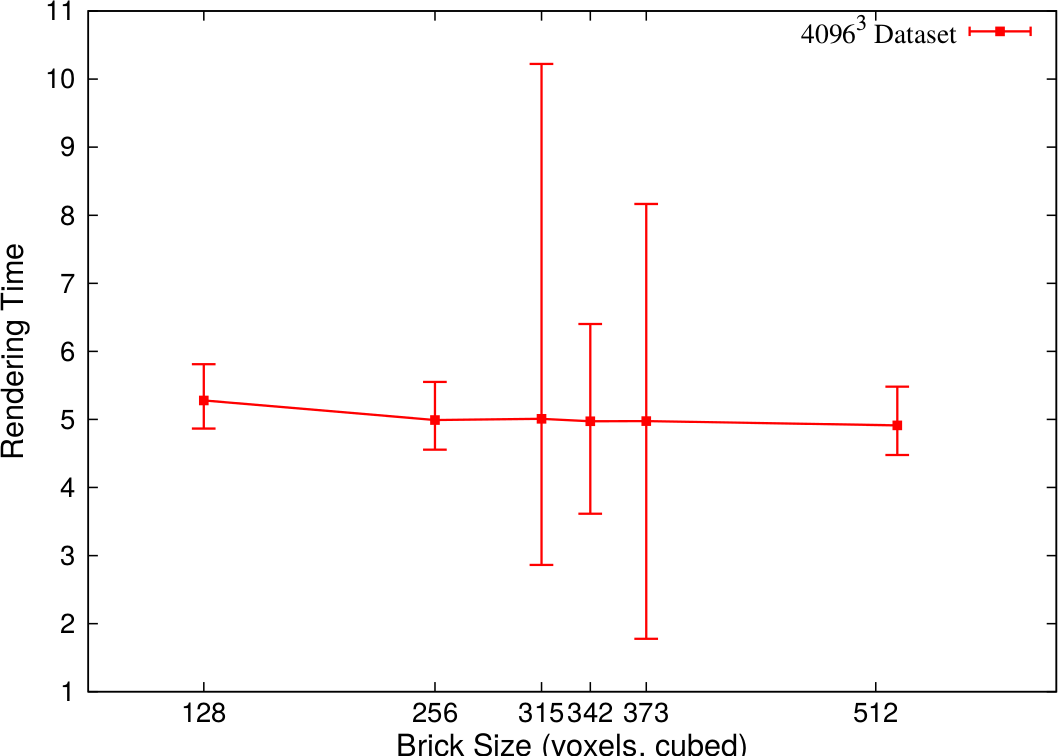
\includegraphics[width=\linewidth]{images/multiscale/bsize}

  \caption{Rendering time as a function of brick size.  Error bars
  indicate the minimum and maximum times recorded, across all nodes,
  for that particular brick size; high diswparity indicates the
  rendering time per-brick was highly variable, and load imbalance
  was therefore likely.  All tests were done with a $4096^3$ data
  set statically laod balanced across 128 GPUs on 64 nodes, using a
  scripted camera that requested the same viewpoints each run.  Note
  that the choice of brick size matters little in the average case, but
  bricks using non-power-of-two sizes give widely varying performance.
  Though raw data shows it is only hundreths of a second faster than
  $256^3$.}
  \label{fig:bsize}
\end{figure}

As can be seen in Figure~\ref{fig:bsize}, the brick size
\emph{generally} has little impact on performance.  A parallel volume
renderer's performance is, however, dictated by the slowest component,
and therefore the average rendering time is less important than the
maximum rendering time.  Taking that into account, it is clear that
brick sizes that are not a power of two are poor choices.  Dropping
down to $128^3$, we can see that per-brick overhead begins to become
noticeable, impacting overall rendering times.  We found larger bricks
sizes of $512^3$ give the absolute best performance, with $256^3$ a
good choice as well, as the differences are minor enough that they may
almost be considered sampling error.  Of course, such recommendations
may be specific to the GPUs
used in \textit{Longhorn}

We were initially surprised to find that the image resolution, while
relevant, was not a significant factor in the overall rendering
time.  When developing single GPU applications that run on a user's
desktop, our experience was the opposite: that image size does play a
significant role in performance.  We at first thought this was due to
skipping bricks that were `empty' under our transfer function---our
domain is perfectly cubic, yet as is displayed in
Figure~\ref{fig:sample} very little of the domain is actually
visible---but even after changing to a transfer function with no ``0''
values in the opacity map, rendering times changed very little.  We
concluded that the data sizes are so large compared to the number of
pixels rendered that the image size is dwarfed by comparison.

In our initial implementaion on \textit{Lens}, we noticed that we
began to strain the memory allocators while rendering a $3000^3$ data
set, as we approached low memory conditions.  Our volume renderer
automatically accounts for low memory conditions and attempts to free
unused bricks before failing outright.  However, an operating system
will thrash excessively before finally deciding to fail an allocation,
and therefore during the time leading up to a failed allocation,
performance will drop considerably.  Worse, we are working in a large
existing code base, and attempting to manage allocations outside our
own subsystems would prove unwieldy.  As such, we found the original
scheme to be unstable; the rendering system would create memory
pressure, causing other subsystems to fail an allocation in areas where
it may be difficult or impossible to ask our volume renderer to free up
memory.

To solve this problem, we render the data in a true out-of-core
fashion: bricks are given to the renderer, rendered into a framebuffer object,
and immediately thrown away.  One might expect that out-of-core algorithms would
have more per-block overhead and therefore be slower than an in-core algorithm.
As shown in Figure~\ref{fig:ooc}, the out-of-core approach actually
outperforms the analogous in-core approach even when there is
sufficient memory to hold the data set at once.  The reasoning
turned out to be that bricks were searched for in a logarithmic data
structure; the conservative approach taken by the out-of-core algorithm
meant that the container maxed out at a single element, accounting for
a minor performance improvement.

\begin{figure}
  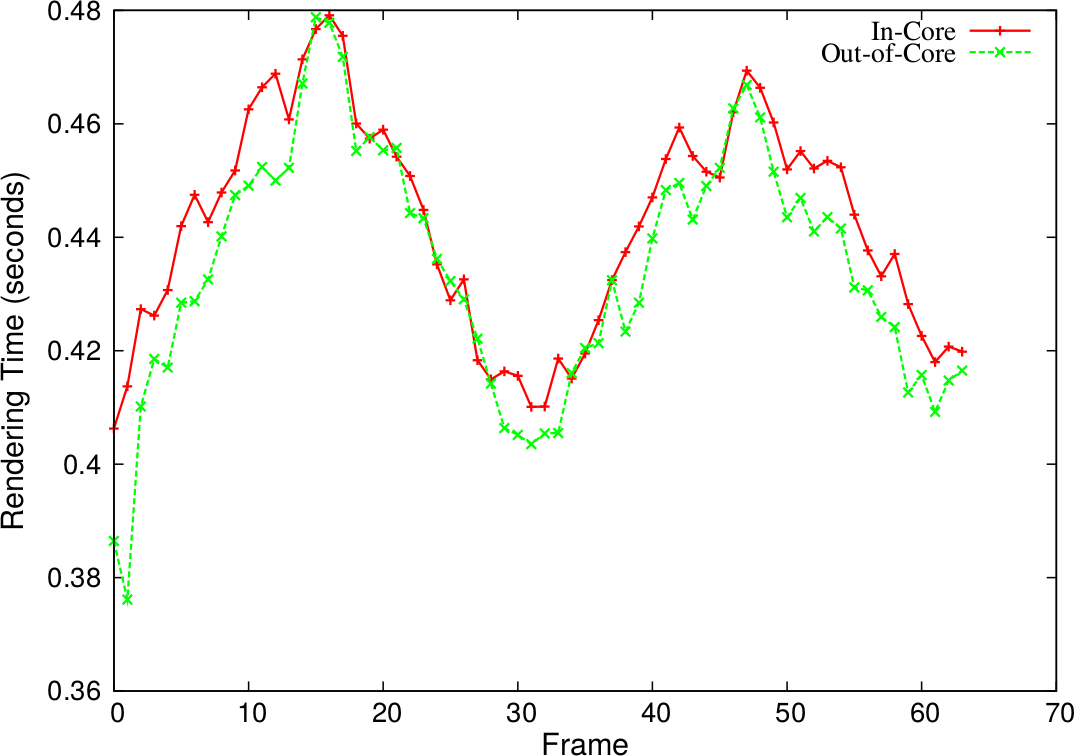
\includegraphics[width=\linewidth]{images/multiscale/ooc}
  \caption{Rendering times, per frame, for the in-core and out-of-core
  approaches to rendering a $1024^3$ data set (which fits comfortably
  in memory) across $16$ GPUs.  Additional processing in the
  out-of-core case doeds not negatively impact performance.}
  \label{fig:ooc}
\end{figure}

\subsubsection{Readback and compositing}

In earlier results, particularly with GPU-based rendering
architectures, the community was generally concerned with the time
required to read the resulting image data from the GPU and into the
host's
memory~\cite{Marchesin:2008:MultiGPU}.  Our study did not provide
corroboration of this concern, which we interpret as a positive data
point with respect to evolving graphics subsystems.  Our system did
demonstrate that this time increased as the resolution grew, but as can
be seen
in Table~\ref{tbl:breakdown}, even at 1024x768 this step took only
thousandths of a second.

\begin{table}
	\begin{tabular}{|c|ccc|c|}\hline
	\textbf{Dataset size} & \textbf{Rendering (s)} & \textbf{Readback (s)} &
		\textbf{Compositing (s)} & \textbf{Total (s)}\\\hline
	$1024^3$ &  0.06141 & 0.00328 & 0.06141 &  0.12610 \\
	$2048^3$ &  0.35107 & 0.00377 & 0.07673 &  0.43157 \\
	$4096^3$ &  2.50984 & 0.00377 & 0.29533 &  2.80894 \\
	$8192^3$ & 19.60648 & 0.00373 & 0.51799 & 20.12820 \\\hline
	\end{tabular}

  \caption{Breakdown of different pipeline stages for various data set
  sizes on 256 GPUs rendering into a $1024 \times 768$ viewport.  All
  times are in seconds.  The $1024^3$, $2048^3$, and $4096^3$ case used
  $13^3$ bricks (varying brick size); the $8192^3$ case used $32^3$
  bricks, making each brick $256^3$ voxels.  Compositing time rises
  only artificially; if a node finishes rendering before other nodes,
  the time it must wait was included under `Compositing' due to an
  artifact of our sampling code.  Thus, the data imply that larger data
  sets see more load imbalance.}

	\label{tbl:breakdown}
\end{table}

The time required for image composition is significantly reduced when
taking advantage of the GPUs available in the visualization vluster.
Since a GPU can render much faster than a software-based renderer, one
can achieve acceptable rendering performance using far fewer nodes.
Compositing, as it scales with the number of nodes involved in the
compositing process, improves significantly by utilizing many fewer
nodes.

\subsection{Load balancing}

We also sought to examine the utility of load balancing algorithms for
our system. We have implemented the algorithms as presented in two
recent parallel volume rendering papers, and compared rendering times
to each other and to a
statically balanced case.  Figure~\ref{fig:balance} illustrates
the comparisons, where the times shown are the maximum across all
processes.

\begin{figure}
  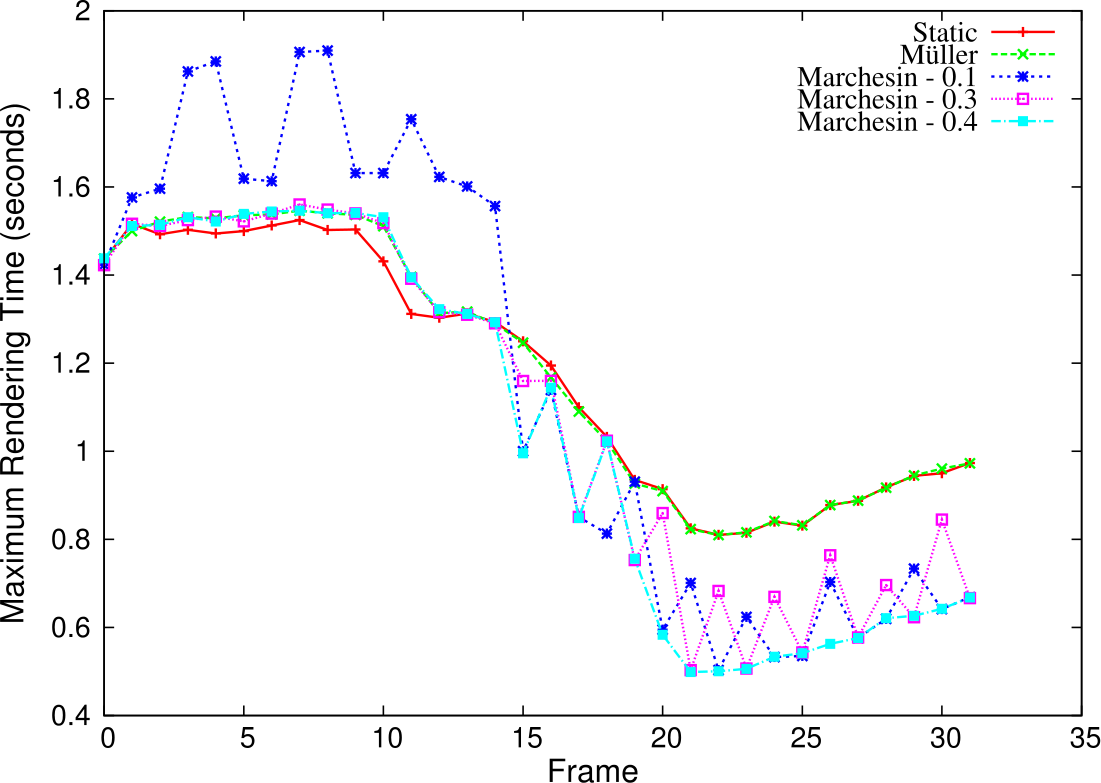
\includegraphics[width=\linewidth]{images/multiscale/balance}
  \caption{The maximum rendering time across all nodes under various
  load balancing algorithms.  The numbers after the `Marchesin'
  algorithms indicate thresholds: rendering disparity under these
  thresholds is ignored.}
  \label{fig:balance}
\end{figure}

We did a variety of experiments with multiple load balancer
implementations, using 8 or 16 GPUs.  Our initiali flythrough dequence
proved to be inappropriate for the application of a load balancer, as
there was not enough imbalance in the system to observe a significant
benefit.  We then attempted to
a `zoom out' flythrough, but rendering times decreasing on \emph{all}
nodes was not a case the the balancers we implemented could effectively
deal with: we found many cases where the balancers would shift data
to a node that was previously idle or at least doing very little
work, and a frame or two later the workload on such nodes would
spike.  This occurred because these nodes had both 1) received new
data as part of the balance and, 2) retained old data as part of the
initial decomposition or previous balancing processes.  The sudden
additional workload of previously invisible bricks caused these nodes
to overcompensate, sending data to other ``idle'' nodes---nodes that
would experience the sample problem in subsequent frames.

In previous work, authors have praised the effect load balancing has
when
zooming \emph{in} to a data set.  This naturally creates imbalance, as
some nodes end up with data that are not rendered under the current
camera configuration, and therefore the node has no work to do.

With the implementations we recreated as faithfully as possible, we did
find that zooming in to the data set was a task that was well-suited
for load balancing.  Still, we encountered issues even with this case.
For the
algorithm given in~\cite{Marchesin:2006:???}, we observed that the
data would move back and forth between nodes quite frequently, having
a negative impact on overall rendering time.  We therefore introduced
a `threshold' parmaeter to the existing algorithm, in an attempt to
limit this `ping-pong' behavior.  As we move up the tree, imbalance
between the left and right subtrees is subject to this threshold; if
it does not exceed the threshold, the imbalance is ignored.  This
is a very useful parameter for ensuring that we do not move data
too eagerly.  Generally, setting this threshold too high will yield
behavior equivalent to the static case; setting it to low leads to a
considerable amount of unnecessary data shifting, and we found that
this in many cases overcompensated for minor, expected variations (such
as those one might expect
from differing brick sizes; see Figure~\ref{fig:bsize}).  For example,
see
Figure~\ref{fig:balance}, in which low thresholds display an obvious
`ping-pong' effect as nodes overcompensate for increased rendering
load.

M\"uller et al. describe a different balancing system~\cite{MSE06}.
This system calculates the average cost of rendering a brick, and
therefore has a clearer idea of what the effect of moving a given set
of bricks will have on overall system performance.  Further, they
introduce additional parameters that add some hysteresis to the system,
and this helped reduce the `ping-pong' effect of nodes sending data
to a neighbor just to receive it in the next frame when the neighbor
becomes overloaded.

We found that this algorithm did do intelligent balancing for
reasonable settings of these parameters, and the additional parametes
could be successfully used to reduce excess data reorganization.  Still
we found two issues with the approach: for one, the assumnption that
`all bricks are equal' did not pan out for our work.  Even assuming
uniform bricks for a data set (true for our case, but likely not in a
general system), one can see in
Figure~\ref{fig:bsize} that the time to render a brick sees variation
on the orde rof a second.  Secondly, despite experimenting with
parameter settings, we found it difficult to get the algorithm to
choose the `best' set of nodes for balancing.  In many cases, we found
a particular node was an outlier, consistently taking the most time
to render per frame.  Yet it was common for this algorithm to balance
different nodes.  While rendering times would generally improve, the
system's performance is determined by the slowest node, and therefore
making the fast nodes faster does not help overall performance.

\begin{figure}
  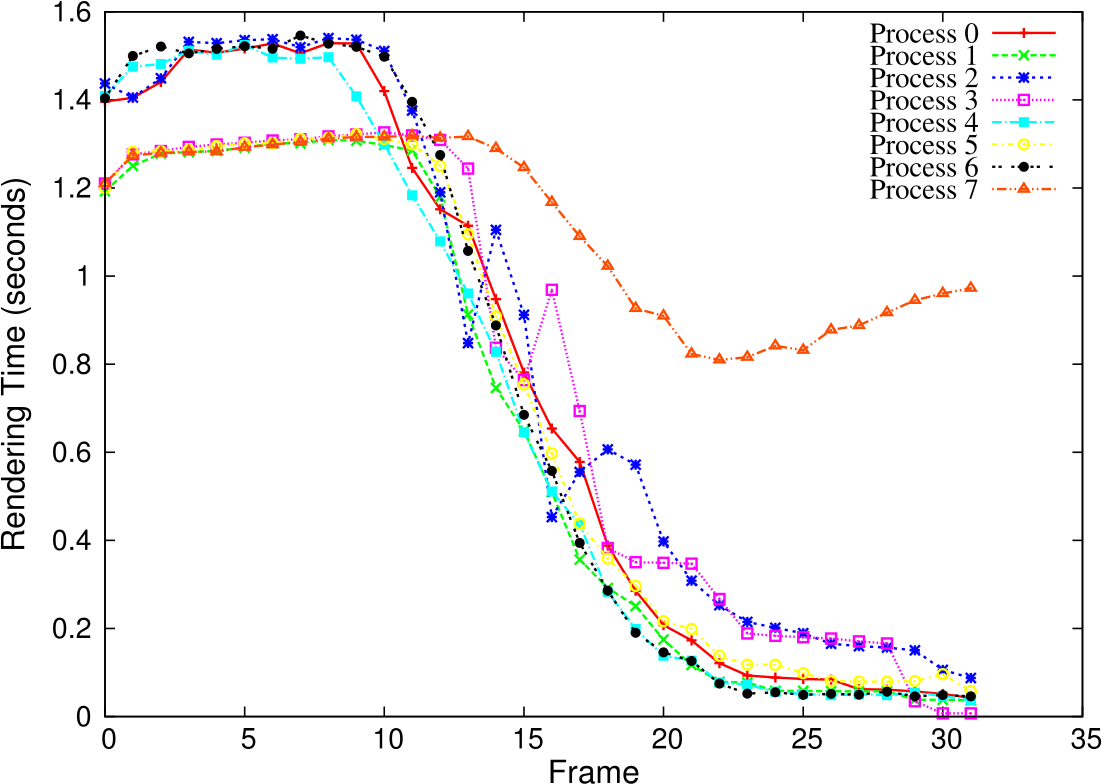
\includegraphics[width=\linewidth]{images/multiscale/mueller}

  \caption{Per-process rendering times for the `M\"uller' line given in
  Figure~\ref{fig:balance}}
  \label{fig:mueller}
\end{figure}

This was apparent in the tests described in Figure~\ref{fig:balance}:
the algorithm balanced between some of the nodes, but the slowest node
was never balanced, and therefore the user-visible performance fror
this run was
equivalenty to the static case.  Figure~\ref{fig:mueller} shows a more
detailed analysis of the execution of the M\"uller algorithm that
generated the data in
Figure~\ref{fig:balance}.  The per-node rendering times in
Figure~\ref{fig:mueller} show that process 7 is usually the last
process to
finish and is often \emph{considerably} slower than the next-to-last.
As evident from the lack of sudden discontinuities in process 7's
rendering times, however, no bricks from process 7 move to other nodes.
Rendering times decrease across other nodes, but the maximum rendering
time does not change.

We theorize that additions to the algorithm to learn weights for each
individual brick would yield friutful results.  Furthermore, the algorithm
explicitly attempts to avoid visiting the entire tree, as an attempt to bound
the maximum time needed to determine a new balancing.  In our work, we did not
observe cases where iterating through nodes in the tree had a measurable
impact on performance, and feel that  by doing so the algorithm could obtain
the global knowledge it needs to balance data effectively.  Both of these
extensions are left for future work.

In Section~\ref{sec:introduction} we noted a variety of quesitons that the
design of our system allows us to answer.

\begin{itemize}

  \item \textit{Rendering vs. compositing}.  As shown in
  Table~\ref{tbl:breakdown}, subsecond rendering times are achieved
  using a very small number of nodes, relative to previous work.  This
  relieves a significant source of work for compositing algorithms.

  \item \textit{Overhead of GPU transfer}.  Table~\ref{tbl:breakdown}
  shows readback time to be on the order of thousandths of a second for
  common image sizes.  Measuring texture upload rates is difficult due
  to the asynchronous nature of OpenGL and current drivers, but we did
  not find evidence to suggest this was a bottleneck.

  \item \textit{Importance of load balancing}.  A dynamic load balancer
  can have a worthwhile impact on perfprmance.  However, it can also
  lower the performance of the system.  Load balancers generally come
  with some number of tunable parameters, and useful settings for
  these parametrs are difficult to determine \textit{a priori}, and
  likely impossible for an end-user to effectively set.  We observed
  that dynamic load balancing for volume rendering struggled in cases
  often encountered in real-world environments and, for this reason,
  believe there is still a gap before deploying these techniques in
  \emph{production} systems.  There is a great opportunity for future
  work in this area.

  \item \textit{Viability}.  As displayed in Figure~\ref{fig:rtime} and
  Table~\ref{tbl:breakdown}, rendering extremely large data sets---up
  to $8192^3$ voxels---is possible on relatively few nodes.  Further,
  data sets up to $2048^3$ can be rendered at an interactive two frames
  per second.

\end{itemize}

\section{Conclusions}
\label{sec:conclusions}

With this study, we demonstrated that GPU accelerated rendering
provides compelling performance for large scale data sets.
Figure~\ref{fig:rtime} demonstrates our system rendering data sets
that are among some of the largest reported thus far, using far fewer
nodes than previous work.  This work shows that a multi-GPU node is a
great fojundational `building block' to compose larger systems cpaable
of rendering very large data.  As the price-performance ratio of a
GPU is better (provided it can effectively parallelize the workload)
than CPU-based solutions, this work makes the case for spending more
visualization supercomputing capital on hardware accleration, and
acquiring smaller yet more performant clusters.

Reports on the time taken for various pipeline stages demonstrate that
PCI-E bus speeds are fast enough that readback performance is not as
great of a concern as it was a few years ago.  Howeever�, it remains to
be seen if contention will become an issue if individual nodes are made
`fatter', utilizing additional GPUs.  The 1 GPU per node given in
Figure~\ref{fig:rtime} suggest that multiple GPUs do contend for
resources, but at this scale the differences are not yet significant
enough for warrant moving away form the more cost-effective `fat'
node architecture.  Given the relatively few nodes needed for good
performance on large data, and external work scaling compositing
worklaod out to tens of thousands of cores, it seems likely that the
relatively `thin' 2-GPU-per-system archietcture can be made to scale
to even larger systems.

We would like to study our system with higher image resolutions, such
as those available on a display wall, and larger numbers of GPUs. At
some point, we expect compositing to become a significant factor in
the amount of time needed to volume render large data, but we have
not approached the cross-over point in this work, due to the use of
`desktop' image resolutions and low numbers of cores.

Our system allows substituting a Mesa-based software renderer when
a GPU is not available. This provided a convenient means of
implementation for an existing large software system, in particular
because it allows pipeline execution to proceed unmodified through
the rendering and compositing stages. However, tests very quickly
showed that using software renderers when a GPU was available was
not worthwhile, and usually ended up hurting performance more than
helping. Therefore, we traded access to more cores for the guarantee
that we will obtain GPUs for each core we do get.

An alternate system architecture would be to decouple the rendering
process from the other work involved in visualization and analysis,
such as data I/O, processing, and other pipeline execution steps. In
this architecture, all nodes would read and process data, but
processed, visualizable data would be forwarded to a subset of nodes
for rendering and compositing. The advantage gained is the ability to
tailor the available parallelism to the visualization tasks of data
processing and rendering, which, as we have found, can benefit from
vastly different parallel decompositions. The disadvantages are the
overhead of data redistribution, and the wasted resources that arise
from allowing non-GPU processes to sit idle while rendering.

Our compositing algorithm assumes that the images from individual
processors can be ordered in a back-to-front fashion to generate the
correct image. For this paper, we met this requirement by using regular
grids, which are easy to load balance in this manner. It should be
possible to also handle certain types of curvilinear grids and perhaps
AMR grids.  Extensions to handle unstructured grids would be difficult,
but represent an interesting future direction.

Load balancing is an extremely difficult problem, and we have just
scratched the surface here. The principal difficulty in load balancing
is identifying good parameters to control how often and to what extent
the balancing occurs. We would like to see ideas and algorithms
which move in the direction of user-friendliness: determining the
most relevant parameters and deriving appropriate values for them
automatically.
